\section{Methodology} \label{isect2}
\subsection{Existing approaches and related literature}
The main economic theory to study sustainable livelihoods was developed by \cite{chambers1992sustainable} who contends that a sustainable livelihood is one that can withstand stress and shock, maintain or improve its assets and capabilities, and create opportunities for future generations to live sustainably. It also should generate benefits for other livelihoods both locally and globally as well as over the long term. The author created the Sustainable Livelihood Approach (SLA) for the purpose of evaluating various vulnerability contexts to improve the effectiveness of development cooperation. The Sustainable Livelihood Framework (SLF) was proposed with a particular emphasis on the institutional processes which mediate the ability to carry out combination of livelihood strategies with the given livelihood resources in a particular context to achieve an outcome. Some of the well-known livelihood frameworks are those proposed by Department of International Department \cite{dfid1999sustainable}, \cite{ellis1999rural} and \cite{scoones2013livelihoods}.\par

\cite{dfid1999sustainable} defines livelihoods broadly and systematically, considering the various assets that individuals or communities can draw upon for sustainable living. It emphasizes the inter-linkage of various capitals (Human, Social, Financial, Physical, and Natural Capital) the households possess with the livelihood outcomes. The framework provides a holistic viewpoint by taking into consideration the dynamic exchange of the capitals and how they influence the result of livelihood. \cite{ellis1999rural}  builds on the DFID model by introducing the idea of vulnerability and emphasizes the importance of understanding the factors that makes certain people or groups more vulnerable to shocks and stresses. The author highlights the significance of understanding the elements that make people or communities more vulnerable to shocks and pressures and presents the idea of vulnerability as a major predictor of livelihood strategies and results. \cite{scoones2013livelihoods} contributed to SLF issue by emphasizing the importance of social relations and political economy in determining the livelihoods. The author's work highlights the need for critical analysis of social relations and political context and how they impact the household's ability to secure more sustainable livelihoods. The framework stress the need for a comprehensive understanding of livelihoods, taking into consideration not only the assets and vulnerability but also the the social, economic and political dimension.\par

In a nutshell, DFID framework provides a comprehensive overview of various capitals that impact livelihoods. It acknowledges the concept of vulnerability but doesn't make it a central focus. Also, it does not explicitly delve into social and political dimension of livelihoods. Ellis on the other side of the spectrum, introduces the concept of vulnerability and places a strong emphasis on understanding the elements that increase the likelihood of failure. The framework includes some consideration of political and institutional factors but is centered more on vulnerability. Scoone highlights the critical role of political economy and power structures in shaping the livelihoods. Each framework brings unique perspectives to the understanding of sustainable livelihoods, with varying levels of focus on capitals, vulnerability, political economy, and power dynamics.\par

\subsubsection{Household Vulnerability Index}
Vulnerability is a concept applied across various disciplines, including engineering, ecology, economics, psychology, and sociology \citep{fang2016rural}. It refers to a state of insecurity when something harmful occurs \citep{chambers1989editorial, chambers2006vulnerability} and is derived from the Latin word "vulnerare" \citep{calvo2005measuring}. Household vulnerability is a complex and multifaceted concept that requires identifying both the threat and the resilience of a person, household, community, or system \citep{zhang2020capital}. Resilience is the ability of a person, household, community, or system to adapt over time to shocks and proactively lower the risk of future shocks \citep{bernier2014resilience}. Studies have shown that household capitals, including financial, human, natural, physical, and social capital, are important determinants of household vulnerability \citep{gaisie2021complexity, zhang2020capital}. The more resilient a system, the less vulnerable it is. Studies have found that less vulnerable households exhibit resilience through alternative livelihoods and social connections \citep{antwi2013characterising}. The multidimensional nature of vulnerability encompasses social, economic, physical, institutional, environmental, and attitudinal factors\citep{rahman2023households, notenbaert2013derivation}.

Numerous studies have been conducted to assess vulnerability in Nepal. Study by \cite{aksha2019analysis} used the Social Vulnerability Index (SoVI) to investigate social vulnerability. The study finds high vulnerability in areas with Dalit and Minority populations. Another study estimated Nepal's vulnerability to poverty using a three-stage feasible generalized least square technique, finding a 33 percent vulnerability \citep{shahiestimating}. The vulnerability score is notably high for minority populations, with Karnali and Sudurpaschhim regions having a higher proportion of highly vulnerable households. In a slight different vein \cite{bista2019grasping} found that a majority of households are sensitive to climate-induced disasters due to their socio-economic status and food insufficiency. A mixed-method approach using the Livelihood Vulnerability Index (LVI) at the community level revealed significant spatial variation in vulnerability, even within the lowest administrative units. A study based on Hindu Kush Himalayas (HKH) found that Khotang district showed the highest multidimensional livelihood vulnerability, with 96.7\% of the population being multidimensionally vulnerable to change \citep{gerlitz2017multidimensional}.

To identify the different levels of vulnerability amongst the households in rural households in our datasets, we construct the Household Vulnerability Index (HVI). Taking into the capitals that households possess, we construct an aggregated index which helps to identify the vulnerable households within the community. The capitals we use to construct the index are: Human; Physical; Social; Financial; and livelihood strategies. To ensure the comparability of indicators that were used in the construction of the household vulnerability index, all indicators were standardised following the \citep{watkins2007human} procedure of standardising indicators for life expectancy index. This ensures that all indicators were normalised to have a relative position between 0 and 1.This method has been widely used in the literature related to vulnerability assessment. \cite{fang2016rural, antwi2013characterising, karunarathne2020developing, huynh2018multi, dumenu2020social} are some of the literature that have employed mini-max/maxi-min normalization technique to construct the vulnerability index.\par

All variables with different scales are normalized with the following Min-Max standardization 
(Equations 1 and 2). Min-Max normalization helps to resize/rescale all variables analogously 
(i.e., into one scale). Here, all values are scaled between 0 and 1. Equation (1) applies to 
variables which have has upward functional relationship with vulnerability, while equation (2) applies to variables which have downward functional relationship with vulnerability.\par  

\begin{align}
	\text{X}_{\text{ij}} &= \frac{X_{\text{i}} - X_{\text{Minj}}}{X_{\text{Maxj}} - X_{\text{Minj}}} \tag{1} \\[1cm] 	
	\text{X}_{\text{ij}} &= \frac{X_{\text{Maxj}} - X_{\text{i}}}{X_{\text{Maxj}} - X_{\text{Minj}}} \tag{2}
\end{align} 
where X is the observed value of the variable related to household i in district j, and Xmax and Xmin are 
maximum and minimum values of each variable, respectively. After normalizing all variables, 
we used equation (3) to calculate the final normalized index for each key component.
\begin{align}
	\text{HVI}_{\text{Cij}} &= \frac{1}{n}\sum_{i=1}^{n}\text{X}_{\text{ij}} \tag{3}
\end{align}
where $\text{HVI}_{\text{Cij}}$ is one of the five key components for HH. The main elements include human capital (C1), physical capital (C2), social capital (C3), livelihood (C4) and financial capital (C5). 	$\text{index}_{\text{Hvi}}$
depicts the variables of the key component indexed by C for i household in j district (while n represents the number of variables for each component). We used equation (4) to 
calculate the overall Hvi for the HH.
\begin{align}
	\text{HVI}_{\text{ij}} &= \sum_{i=1}^{n}\text{HVI}_{\text{Cij}} \tag{4}
\end{align}
where HVI is the Multi-facet Composite Household Vulnerability Index for HH x. 
C represents the numbers of key components,  indicates the weighting schemes used for the 
composite index, and n ensures the number of key components. Table 3 illustrates the weighting 
schemes used for the composite index calculated.\par 
                                   
\subsection{Household Vulnerability and Environmental Dependence}
After we construct the index and identify the most and least vulnerable households, we attempt to understand the effects of the variables that is likely to influence the vulnerability index. These variables represent the liability to a household. Environmental income, a semi-capital/semi-liability characteristic variable, represents the revenue a household generates from forest and non-forest sources. Dependence in this livelihood strategy can be a capital source for rural households with limited resources, but also a liability in the context of climate change and environmental degradation. The study investigates the influence of environmental dependence on household vulnerability.\par

To examine the effect of Environmental dependence on Household vulnerability, this study employs panel estimation techniques, including pooled-OLS, fixed effects (FE), and random effects (RE) models. While simple pooled-OLS doesn't account for the time-specific or hosuehold-specific effects, the fixed effects and random effects models are designed to address such endogenity issues. Pooled-OLS is essentially a statistical regression analysis method that visually represents the relationship between data points and determines the best-fit line for a dataset. However, the fixed effects model is theoretically more suitable for cases involving unobservable individual  or household effects that may be correlated with the variables included in the model. Conversely, if individual effects are strictly uncorrelated with explanatory variables, the random effects model is a preferable choice \citep{hsiao2022analysis}.   Effect of Environmental dependence on household vulnerability is modeled using
following regression,
\vspace{-\baselineskip}
\begin{center}
	\begin{align}
		\mathit{HVI}_{i,t} &= \beta_{0} + \delta \mathit{\mathbf{ED}_{i,t}} + \mathbf{X}_{i,t} \beta + \mathbf{Z}_i \lambda + \mathbf{T}_t \delta_t + \boldsymbol{\epsilon}\tag{5}
	\end{align}
\end{center}
where, \textit{HVIi,t} is Household Vulnerability of $i^{th}$ household in \textit{t} year, \textit{EDi,t} is Environmental dependence, \textit{T} is year control variable, \textit{Xi,t} is the variables controlled for, which includes Dependency ratio, log of debt, count of shock experienced and \textit{Zi,t} represents control for time invariant
fixed effect such as district and VDCs and $\beta_{0}, \delta, \beta, \lambda, \delta_t$ are the parameter of the model.\par 

\subsection{Diagnostic Tests}

For each techniques of the Panel data analysis, we'll run few diagnostic tests to check for the effects to be included in the model such as Individual and Time effects. Also, we run the efficiency test for choosing between the models.\par 

\subsubsection{Individual Effects Test} 
We run the Pooled Ordinary Least Squares (OLS) regression model without considering individual effects. After obtaining the results from Pooled OLS regression, we conduct F-test to determine if there are significant individual effects (fixed effects) present in the model. We'll refer to the F-statistic and associated P-value to determine the presence of significant individual effects.  A low p-value suggests the presence of significant individual effects.\par 

\subsubsection{Time Fixed Effects Test}
We also test for if there are time effects in the model. For this, we run the Pooled Ordinary Least Squares (OLS) regression model without considering individual effects. After obtaining the results from Pooled OLS regression, we conduct the Lagrange Multiplier Test - \cite{honda1988size}. It will allow us to determine if there are significant time effects (fixed effects) present in the model. We'll refer to the t-statistic and associated P-value to determine the presence of significant individual effects.  A low p-value suggests the presence of significant time effects.\par 

\subsubsection{Breusch-Pagan Lagrange Multiplier (BPLM) Test}
This test is commonly referred to as Pool-ability test conducted for confirming if the cross-sectional unit in the panel has the same intercept or a different intercept. \cite{breusch1980lagrange} assesses the pool-ability of the data after incorporating the time and individual fixed effects. We'll analyze the test-statistic and associated p-value. A low p-value suggests that the data is not poolable, indicating the inadequacy of Pooled OLS regression. We'll go for Random effects (RE) regression if the p-value is low.

\subsubsection{Hausman Specification Test}
If the BP-LM test suggests that the data is not pool-able and suggests to go for Random Effects (RE) model, we'll run the RE regression. We'll also run the Fixed effects (FE) model to compare the result. After running both Random Effects (RE) and Fixed Effects (FE) models, conduct the Hausman Specification test \cite{hausman1978specification} to determine the efficient model. The test is to check whether the coefficients estimated by the two models are significantly different. We'll analyze the test statistic, typically a chi-square value, and assesses the associated p-value.\par 

\subsection{Data sources}
This study employs the A unique environmental augmented household-level livelihood panel dateset \citep{walelign2022unique} from
Nepal, Full Panel 2006-2012, produced by Tribhuvan University’s Institute of Forestry and the University of Copenhagen’s Department of Food and Resource Economics . It is a geographically representative survey spanning three main physio-graphic regions of Nepal. Data was collected in the districts of Chitwan (lowland), Kaski (mid-hills), and Mustang (mountains). Total of 507, 446 and 428 randomly sampled households were surveyed in the year 2006, 2009 and 2012 respectively. For the questionnaire (see \cite{larsen2014role}). \par

\begin{figure}[htb] 
	\centering
	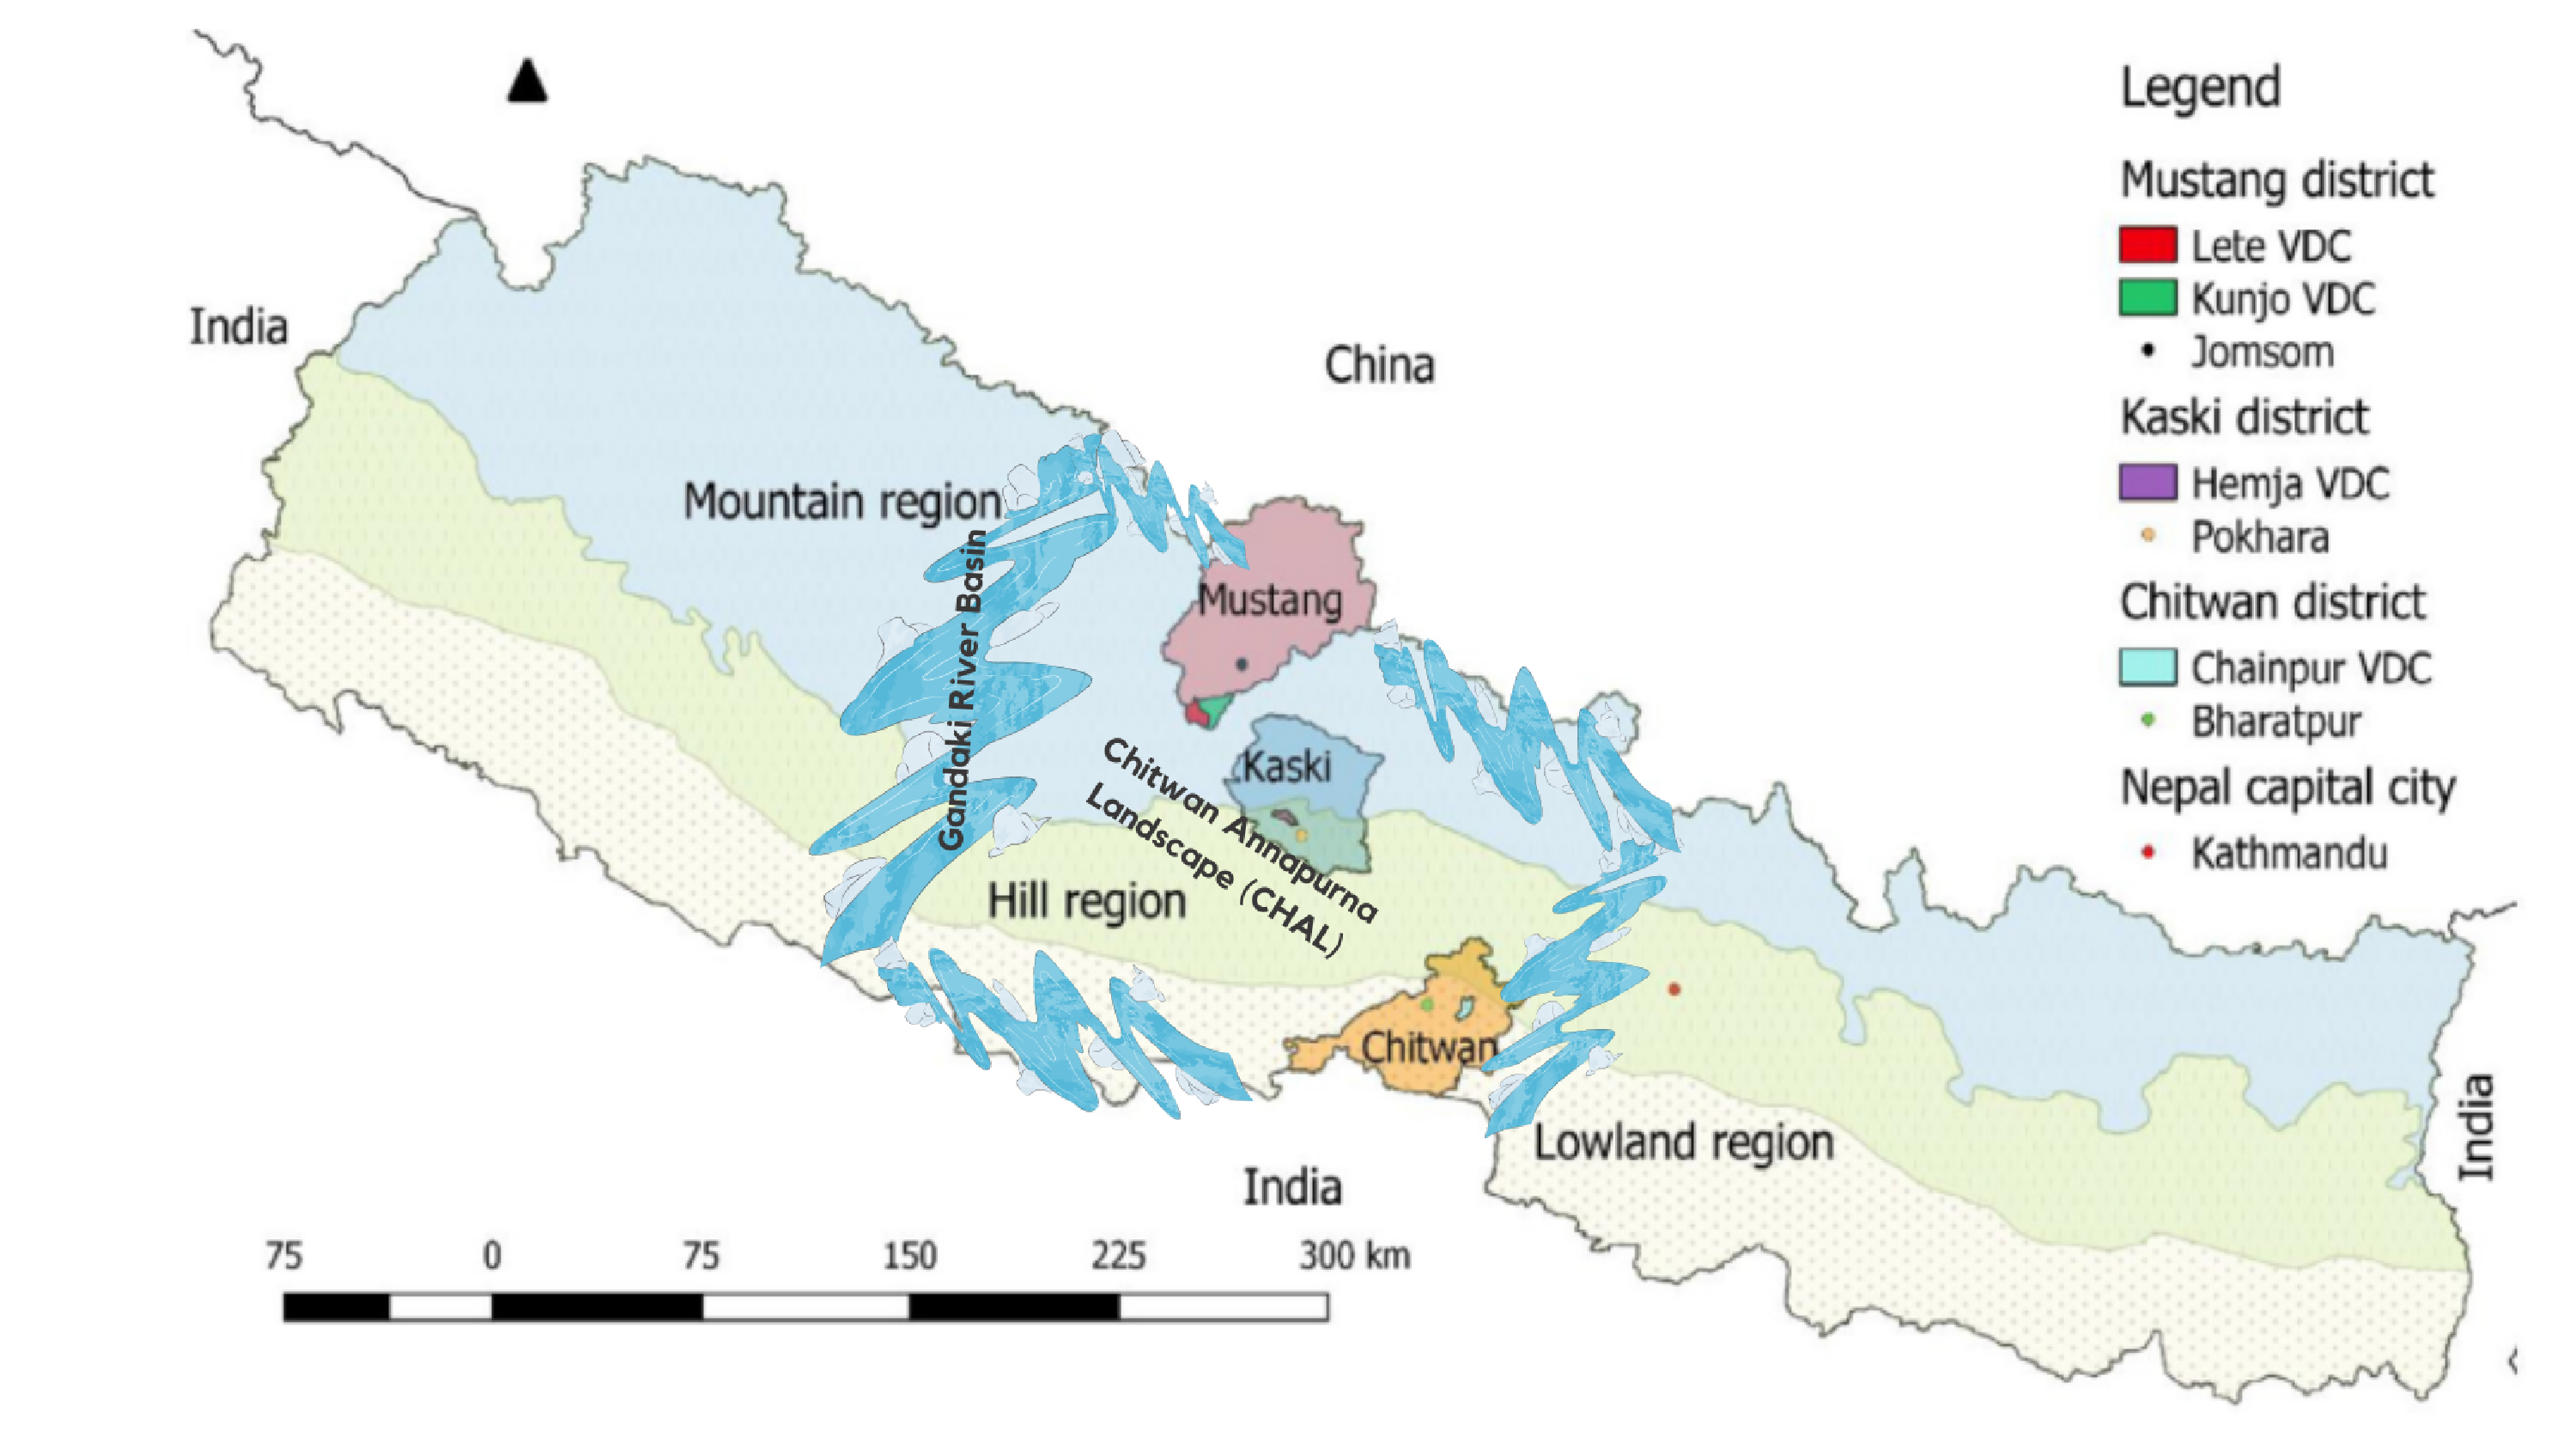
\includegraphics[scale=0.31]{./figure/Study site}
	\caption{Changes in real wage throughout the wage distribution (1998-2018)}
	\label{fig:wagechangeAll}
\end{figure} 

The three primary physio-graphic regions of Nepal—the lowlands, mid-hills, and mountains—are covered by the study sites. The selection factors included the following: (i) Nepal's changes in elevation and vegetation; (ii) the environmental reliance of households; (iii) the attitudes of communities toward long-term research; and (iv) village accessibility and researcher safety (because of the ongoing civil conflict in Nepal at the time of site selection in 2005).\par
The data was collected through the Community Based Forest Management in the Himalaya
(ComForM) phases I - III collaborative project conducted by the Institute of Forestry (IOF) at Tribhuvan University and the Department of Food and Resource Economics (IFRO) at the University
of Copenhagen, with support from the Department of Forest Research and Survey (DFRS) at the
Ministry of Forests and Soil Conservation, Nepal. The questionnaire design was developed together with the Poverty Environment Network (PEN).\par  

 
                            
